%%%%%%%%%%%%%%%%%%%%%%%%%%%%%%%%%%%%%%%%%%%%%%%%%%%%%
%			ŠABLONA PÍSNIČEK v. 18.09               %
%%%%%%%%%%%%%%%%%%%%%%%%%%%%%%%%%%%%%%%%%%%%%%%%%%%%%
% Tento soubor slouží jako (naučná) šablona, pomocí 
% které lze vytvářet zdrojové soubory k jednotlivým 
% písním.
%%%%%%%%%%%%%%%%%%%%%%%%%%%%%%%%%%%%%%%%%%%%%%%%%%%%%
%			Jak psát soubory songů?                 %
%%%%%%%%%%%%%%%%%%%%%%%%%%%%%%%%%%%%%%%%%%%%%%%%%%%%%
%	1. Text písně se začíná psát na místě START 
%	   a končí na místě END. Zbylý text ignorujte.
%	2. Jak bude vypadat pdf písně zjistíte po tom, 
%	   co soubor zkompilujete pomocí souboru   
%      ../Generator/generator. 
%	3. Při psaní dodržujte následující TeX pravidla:
%	 a) Nový řádek napíšete pomocí dvou odsazení 
%	    tedy dvou enterů.
%	 b) Nová sloka se píší pomocí \sloka a odsazení.
%		Refrén se píše jako \refren, v případě více 
%		refrénů \refren[č. refrénu].
%	 c) Akordy se píšou tak, že napíšete před slovo,
%	    kde chcete mít akord (bez mezery):
%		^{AKORD1\,AKORD2...}.
%	4. Pokud chcete ušetřit tvůrcům práci, tak 
%	   si přečtěte další poučný soubor o typografii 
%	   ../../Typo_pravidla.txt.
%	5. Akordy stačí psát jen do první sloky, když 
%	   se nezmění -- kytaristé to zvládnou
%	7. Název písně pište na místo [NÁZEV] a autora 
%	   pište na místo [AUTOR] 
%	7. Jak psát věci na české klávesnici:
%	   \ = alt gr + q; [/] = alt gr f/g; 
%      {/} = alt gr + b/n; ^ = alt gr + 3 , cokoliv
%%%%%%%%%%%%%%%%%%%%%%%%%%%%%%%%%%%%%%%%%%%%%%%%%%%%%
%			Jak kompilovat jednotlivé písně?        %
%%%%%%%%%%%%%%%%%%%%%%%%%%%%%%%%%%%%%%%%%%%%%%%%%%%%%
%	1. Více návodu je k tomuto napsáno v souboru 
%      ../Generator/generator. 
%%%%%%%%%%%%%%%%%%%%%%%%%%%%%%%%%%%%%%%%%%%%%%%%%%%%%
%			Jak kompilovat celý zpěvník?			%
%%%%%%%%%%%%%%%%%%%%%%%%%%%%%%%%%%%%%%%%%%%%%%%%%%%%%
%	1. Více návodu je k tomuto napsáno v souboru
%	   ../Cely_zpevnik/zpevnik.tex.
%%%%%%%%%%%%%%%%%%%%%%%%%%%%%%%%%%%%%%%%%%%%%%%%%%%%%
\begin{song}{title=\predtitle \centering Wonderwall \\\large Oasis }  %% sem se napíše jméno songu a autor

\vspace*{.5cm}

\begin{centerjustified}
\vetsi

\predehra
\textbf{$4\times$ Em G D A7sus4}


\sloka
^{Emi\z}Today is ^{G\z}gonna be the day

That they're ^{D\z}gonna throw it back ^{A7sus4}to~you.

^{Emi\z}By now you ^{G\z}should've somehow

^{D}Realised what you ^{\z A7sus4}gotta~do.


^{Emi}I~don't believe that ^{G\z}anybody

^*{D}Fee ls the ^*{A7sus4}way~I~do~abo ut you now.  ^{D A7sus4}


\sloka
Backbeat the word is on the street

That the fire in your heart is out.

I'm sure you've heard it all before

But you never really had a doubt.

I don't believe that anybody feels

The way I do about you now.



\refren[1]
And ^{C}all the roads we ^*{D}hav e to walk ^{\z Emi}are winding

And ^{C}all the lights ^{\z D}that lead us there ^*{Emi}are~bl inding

^*{C}The re are many ^*{D}thi ngs that I would

^{Emi\z}Like to ^{D G\z}say~to you

But I ^*{D}don 't ^{\z A7sus4}know how.


\end{centerjustified}
\newpage
\begin{centerjustified}

\refren[2]
Because ^*{C}may be ^{Emi G}

You're ^{Emi}gonna be the one that ^{C\z}saves me? ^{Emi G}

And ^{Emi}after ^{C\z}all ^{Emi G Emi}

You're my ^*{\z C}wonderwal l. ^{Emi G Emi G}

\sloka
Today was gonna be the day

But they'll never throw it back to you.

By now you should've somehow

Realised what you're not to do.

I don't believe that anybody

Feels the way I do

About you ^{Emi}now.~ ^{G D A7sus3}

\refren[2]
I said maybe

You're gonna be the one that saves me?

And after all

You're my wonderwall.

\refren[2]
I said maybe (I said maybe)

You're gonna be the one that saves me?

And after all

You're my wonderwall.

I said maybe. (I said maybe)

/: You're ^{Emi}gonna be the one that ^{C\z}saves me? (that ^{Emi \z}saves ^{\z G}me) :/

You're gonna be the one that saves me? (that saves me)

\ssloka{\textbf{Sólo:}}\\
\centering
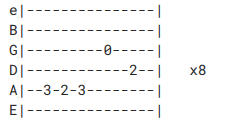
\includegraphics[scale=3]{../taby/wonderwall.png}

\vspace{.5cm}
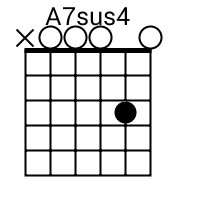
\includegraphics[width=3cm]{../Akordy/a7sus4.png}
\end{centerjustified}
\setcounter{Slokočet}{0}
\end{song}
